\chapter{Modelado de sistemas dinámicos}

\section{Sistemas en el espacio de estados}
Nos vamos a centrar en sistemas que puedan ser descritos por características cuantificables. A estas características las vamos a llamar {\bf estados}, como por ejemplo, una temperatura, una velocidad, o un voltaje. Si estos estados dependen del tiempo, entonces, llamamos {\bf señal} a la sucesión de valores de los estados en el tiempo. Uno podría interaccionar con el sistema a través de una {\bf entrada} cuantificable, y a su vez medir información del sistema a través de una {\bf salida} cuantificable.

Vamos a definir $x(t)\in\mathbb{R}^n$, $y(t)\in\mathbb{R}^m$ y $u(t)\in\mathbb{R}^k$ como el vector apilado de estados, la salida, y la entrada a un sistema $\Sigma$ respectivamente. En particular, son señales, e.g., $x :[0,\infty) \to \mathbb{R}^n$.

El sistema $\Sigma$ es un modelo que predice el valor de los estados y la salida a lo largo del tiempo. Esta predicción incorpora la interacción de la entrada en los estados y la salida. En particular, vamos a emplear ecuaciones diferenciales como herramienta para predecir la evolución en el tiempo de los estados del sistema $\Sigma$ como se muestra a continuación
\begin{equation}
	\Sigma := \begin{cases}
		\dot x(t) =& f(x(t),u(t)) \\ y(t) =& g(x(t),u(t))
	\end{cases}, 
\label{eq: sigma}
\end{equation}
en donde $\dot x := \frac{\mathrm{d}}{\mathrm{dt}}(x(t))$ es la notación para la derivada total con respecto del tiempo, y $f: \mathbb{R}^n \times \mathbb{R}^k \to \mathbb{R}^n$ y $g: \mathbb{R}^n \times \mathbb{R}^k \to \mathbb{R}^m$ son funciones.

Podemos representar el sistema $\Sigma$ como un bloque con puertos de entrada y de salida como se muestra en la figura \ref{fig: sigma}.

\begin{figure}[!h]
\centering
\begin{tikzpicture}[auto, node distance=2cm,>=latex']
	\node [input, name=input] {};
	\node [block, right of=input] (system) {$\Sigma$};
	\node [output, right of=system] (output) {};
	\draw [draw,->] (input) -- node {$u(t)$} (system);
	\draw [->] (system) -- node [name=y] {$y(t)$}(output);
\end{tikzpicture}
	\caption{Diagrama de bloque entrada/salida del sistema $\Sigma$.}
	\label{fig: sigma}
\end{figure}

\section{Ejemplos}
\subsection{Péndulo invertido}

Vamos a derivar las funciones $f$ y $g$ en (\ref{eq: sigma}) para el sistema del péndulo invertido.

Primero, vamos a hallar la ecuación diferencial que describe la dinámica de una masa $m\in\mathbb{R}_+$ en el extremo de un péndulo de longitud $l\in\mathbb{R}_+$ tal y como se muestra en la figura \ref{fig: invpen}. Vamos a considerar que podemos interactuar con el sistema por medio de un torque $T\in\mathbb{R}$ en el otro extremo del péndulo, que la masa sufre un rozamiento proporcional $b\in\mathbb{R}_+$ a su celeridad, y que podemos medir el ángulo $\theta\in\mathbb{R}$ que forma el péndulo con la vertical.

\begin{figure}[!h]
\centering
\begin{tikzpicture}
    \coordinate (origo) at (0,0);
    \coordinate (pivot) at (1,5);

    % draw axes
	\fill[black] (origo) circle (0.05) ++ (-0.25,0.25) node (T) [black] {$T$} ++(0.75,0.75) node (l) [above] {$l$};
    \draw[thick,gray,->] (origo) -- ++(4,0) node[black,right] {$x$};
    \draw[thick,gray,->] (origo) -- ++(0,4) node (mary) [black,above] {$y$};

    % draw roof
    \fill[pattern = north east lines] ($ (origo) + (-1,0) $) rectangle ($ (origo) + (1,-0.5) $);
    \draw[thick] ($ (origo) + (-1,0) $) -- ($ (origo) + (1,0) $);

    \draw[thick] (origo) -- ++(-300:3) coordinate (bob) ++(0.5,0) node (hola) [black] {$m$};
    \fill (bob) circle (0.2);
    \draw[->] (bob) -- ++(0,-1) node (mg) [right] {$mg$};
    \draw[->] (bob) -- ++(-0.5,0.5) node (fr) [above] {$b\dot\theta$};

    \pic [draw, <-, "$\theta$", angle eccentricity=1.5] {angle = bob--origo--mary};
\end{tikzpicture}
\caption{Inverted pendulum}
\label{fig: invpen}
\end{figure}

Define $g = 9.8$ y $I\in\mathbb{R}_+$ como la aceleración gravitatoria y el momento de inercia del péndulo respectivamente. Es sencillo comprobar que $I = ml^2$, y explotaremos que $I \ddot\theta = \text{suma de torques}$. De hecho, tenemos que considerar tres torques: 1. Torque $T$ ejercido por nosotros en la base del péndulo; 2. Torque $-bl\dot\theta$ ejercido por la fricción en la masa; 3. Torque $mgl \sin\theta$ ejercido por la atracción gravitatoria. Por lo que la ecuación diferencial que modela el comportamiento del péndulo invertido es
\begin{equation}
\ddot\theta = \frac{1}{ml^2}\left(mgl\sin{\theta}-bl\dot\theta + T\right).
\label{eq: dyn}
\end{equation}

Parece razonable escoger $\theta$ como uno de los estados para construir $x(t)$ en (\ref{eq: sigma}). De hecho, la ecuación (\ref{eq: dyn}) es de segundo orden en $\theta$, por lo que es conveniente escoger $\dot\theta$ como un estado también. Por lo tanto, definamos nuestro vector de estados como
\begin{equation}
x := \begin{bmatrix}\theta \\ \dot\theta \end{bmatrix},
\end{equation}
y como el torque $T$ es como interactuamos con el sistema, escogemos como entrada $u(t) = T(t)$.

Ahora estamos listos para construir las funciones $f$ and $g$ en (\ref{eq: sigma}) para el péndulo invertido. Atención a que $f$ y $g$ solo toma como argumentos los vectores de estados $x$ y de entradas $u$. En el lado izquierdo de (\ref{eq: sigma}) tenemos la derivada temporal de $x(t)$, por lo que

\begin{equation}
	\frac{\mathrm{d}}{\mathrm{dt}}\left(\begin{bmatrix}\theta \\ \dot\theta \end{bmatrix}\right) = f(x(t), u(t)) = \begin{bmatrix}f_1(x(t), u(t)) \\ f_2(x(t), u(t))\end{bmatrix}, \label{eq: fn}
\end{equation}
donde automáticamente obtenemos que $f_1 = \dot\theta$. Fijarse que la primera fila de $f$ en (\ref{eq: fn}), a la izquierda tenemos que $\frac{\mathrm{d}}{\mathrm{dt}}\theta$, y a la derecha tenemos que $f_1 = \dot\theta$ porque $\dot\theta$ es un estado o elemento de $x$. Desafortunadamente, no podemos decir que $f_2 = \ddot\theta(t)$ porque $ \ddot\theta$ no es un estado o elemento de $x$. No obstante, tenemos que la segunda fila $f_2$ viene dada por la ecuación (\ref{eq: dyn}). Por lo que podemos escribir $f$ como
\begin{equation}
	\frac{\mathrm{d}}{\mathrm{dt}}\left(\begin{bmatrix}\theta \\ \dot\theta \end{bmatrix}\right) =  f(x(t), u(t)) = \begin{bmatrix} \dot\theta \\ \frac{1}{ml^2}\left(mgl\sin{\theta}-bl\dot\theta + T\right) \end{bmatrix}. \label{eq: f}
\end{equation}

El cálculo de $g$ es más sencillo en este caso. Hemos establecido al comienzo que solo podemos medir el ángulo $\theta$. Por lo que $y(t) = \theta(t)$, i.e.,
\begin{equation}
g(x(t),u(t)) =  \theta(t).
	\label{eq: g}
\end{equation}

%A Python simulation of this dynamics can be found at \url{https://github.com/noether/aut_course}.

\subsection{El oscilador de Van der Pol}
Se trata de un oscilador, propuesto por primera vez por Balthasar Van der Pol, cuando trabajaba en Philips, para explicar las oscilaciones observadas en tubos de vacío. Podemos obtener la ecuación del oscilador, empleando el circuito de la figura \ref{fig:vdp}.
\begin{figure}
\centering
\begin{circuitikz}[american, scale = 0.6]\draw
(0,-4)to[short]
(4,-4)to[short,,i^<= $i_C$]
(5,-4)to[short,i=$i_N$]
(6,-4)to[short](10,-4)
(0,-7.5)to[C = C](0,-4)
(5,-4) to[L = L, i>^= $i_L$,*-* ](5,-7.5)
(10,-4) to[generic=NL,  i= $i_N \equiv h(v)$](10,-7.5) 
(0,-7.5)to[short](10,-7.5)
;
\end{circuitikz}
\caption{Circuito eléctrico no lineal}
\label{fig:vdp}
\end{figure}

Donde el elemento no lineal NL, presenta una relación entre voltaje e intensidad caracterizada por la función $h(v)$.

El voltaje $v$ en los tres componentes del circuito debe ser igual; además,
\begin{align}
v = L \frac{di_L}{dt}\\
i_C = C\frac{dv}{dt}
\end{align}
Si aplicamos la primera ley de Kirchohff al nodo superior del circuito,
\begin{align}
i_C+i_L+i_N = 0\\
C\frac{dv}{dt}+\frac{1}{L}\int_{-\infty}^{t}v(s)ds +h(v)=0\label{eq:vdp}
\end{align}
Si derivamos (\ref{eq:vdp}) con respecto al tiempo, dividimos por $C$ y reordenamos,
\begin{equation}\label{eq:vdp2}
\frac{d^2v}{dt^2}  + \frac{1}{C}\frac{dh(v)}{dv}\frac{dv}{dt} + \frac{1}{LC}\cdot v= 0
\end{equation}
Se trata de un caso particular de la ecuación de Liénard,
\begin{equation}
\ddot{v} +f(v)\dot{v}+g(v) = 0
\end{equation}
Si definimos ahora, $h(v)$,
\begin{align}
h(v) = m(\frac{1}{3}v^3-1)\\
\frac{dh}{dv} = m(v^2-1)
\end{align}
y sustituyendo en (\ref{eq:vdp2}),
\begin{equation}
\ddot{v} +m\frac{1}{C}(v^2-1)\dot{v}+\frac{1}{LC}v = 0
\end{equation}

Podemos representarla finalmente en variables de estado, tomando $x_1=v$ y $x_2=\dot{v}$,
\begin{align}
\dot{x}_1 &= x_2\\
\dot{x}_2 &= -\frac{1}{LC}x_1 - m\frac{1}{C}(x_1^2-1)x_2 \label{eq:vdpst2}
\end{align}
Podemos ahora hacer un primer análisis cualitativo. El primer término a la derecha del igual en  la ecuación (\ref{eq:vdpst2}) representa una fuerza recuperadora proporcional al desplazamiento, el segundo término, crecerá con la velocidad para $x_1 < 1$, alejando así al sistema del origen  y representará un término disipativo para $x_1 > 1$ acercándolo por tanto de nuevo al origen. Es por tanto esperable, que se alcance
algún tipo de situación de equilibrio. Más adelante definiremos esta situación rigurosamente como un ciclo límite. 
\subsection{Un vehículo de cuatro ruedas. }
La figura \ref{fig:vehir} muestra un esquema de un vehículo terrestre de cuatro ruedas, visto desde arriba. Si consideramos que se mueve en el plano $x,y$, y que su velocidad instántanea $\vec{V}$ está siempre orientada en la dirección de avance del vehículo $psi$--asumimos que no derrapa, ni se mueve lateralmente--, podemos entoces definir el velocidad, en el sistema de referencia $x,y$ como,
\begin{align}
\dot{x} = V_x(t) = V\cos(\psi(t))\\
\dot{y} = V_y(t) = V\sin(\psi(t))\\
\end{align}

\begin{figure}
\centering

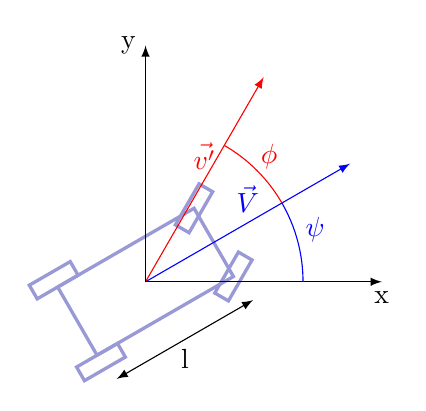
\begin{tikzpicture}
\draw(0,0)[rotate around={30:(0,0)},very thick,draw = blue!60!black!40]rectangle(2,1);
\draw(-0.3,-0.2)[rotate around={30:(0,0)},very thick,draw = blue!60!black!40]rectangle(0.3,0.0);
\draw(-0.3,1)[rotate around={30:(0,0)},very thick,draw = blue!60!black!40]rectangle(0.3,1.2);
\draw({2*cos(30)-0.3},{2*sin(30)-0.1})[rotate around={60:({2*cos(30)},{2*sin(30)})},very thick,draw = blue!60!black!40]rectangle({2*cos(30)+0.3},{2*sin(30)+0.1});
\draw({2*cos(30)-sin(30)-0.3},{2*sin(30)+cos(30)-0.1})[rotate around={60:({2*cos(30)-sin(30)},{2*sin(30)+cos(30)})},very thick,draw = blue!60!black!40]rectangle({2*cos(30)-sin(30)+0.3},{2*sin(30)+cos(30)+0.1});
\draw[blue]({cos(30)-0.5*sin(30)},{sin(30)+0.5*cos(30)})--node[above]{$\vec{V}$}({4*cos(30)-0.5*sin(30)},{4*sin(30)+0.5*cos(30)})[-latex];
\draw[red]({cos(30)-0.5*sin(30)},{sin(30)+0.5*cos(30)})--node[above]{$\vec{v'}$}({cos(30)-0.5*sin(30)+3*cos(60},{sin(30)+0.5*cos(30)+3*sin(60})[-latex];

\draw({cos(30)-0.5*sin(30)},{sin(30)+0.5*cos(30)})--({3+cos(30)-0.5*sin(30)},{sin(30)+0.5*cos(30)})[-latex]node[anchor=north]{x};
\draw({cos(30)-0.5*sin(30)},{sin(30)+0.5*cos(30)})--({cos(30)-0.5*sin(30)},{3+sin(30)+0.5*cos(30)})[-latex]node[anchor=east]{y};

\draw[blue]({2+cos(30)-0.5*sin(30)},{sin(30)+0.5*cos(30)})arc(0:30:2);
\draw[red]({3*cos(30)-0.5*sin(30)},{3*sin(30)+0.5*cos(30)})arc(30:60:2);
\draw[blue]({3.2*cos(30)},{3.2*sin(30)}) node[]{$\psi$};
\draw[red]({3.4*cos(50)},{3.3*sin(50)}) node[]{$\phi$};
\draw[latex-latex](0.25,-0.3)--node[below]{l}({2*cos(30)+0.25},{2*sin(30)-0.3});
\end{tikzpicture}
\caption{Esquema de un vehículo terrestre de 4 ruedas}
\label{fig:vehir}
\end{figure}

Además el vehículo girará, siempre que las ruedas delanteras no estén alineadas con las ruedas traseras, cambiando así su dirección de avance . Podemos relacionar la velocidad de giro del vehículo $\dot{\psi}$ con el ángulo de orientación de las ruedas delanteras $\phi$, y la velocidad a la que avanzan $\vec{v'}$.  podemos obtener las componetes de dicha velocidad en ejes cuerpo (paralela y perpendicular a la dirección de avance del vehículo),

\begin{align}
v_{P} = v'\cos(\phi(t))\\
v_{T} = v'\sin(\phi(t))
\end{align} 

Pero la rueda esta unida al vehículo así que su velocidad en la direccíon de avance debe ser la misma que la del vehículo: $v_P \equiv V$.  A partir de esta relación podemos obtener la velocidad tangencial de las ruedas como,
\begin{equation}
v_T = V\frac{\sin(\phi)}{\cos(\phi)} = V\tan(\phi)
\end{equation}

Si tomamos como centro de giro del vehículo el centro de su eje trasero, y la batalla (distancia entre ejes) es $l$, obtenemos una expresión para su velocidad de giro,
\begin{equation}
\dot{\psi} = \frac{V}{l}\tan(\phi)
\end{equation}

En resumen, podemos describir el sistema mediante tres ecuaciones de estado $x_1 \equiv x, x_2\equiv	y, x_3 \equiv \psi$:
\begin{equation}
	\begin{cases}
		\dot x_1 &=  V\cos(x_3)\\  
		\dot x_2 &=  V\sin(x_3)\\
		\dot x_3 &= \frac{V}{l}\tan(\phi)
	\end{cases}
\end{equation}

Si consideramos $V=cte$, la única entrada al sistema sería el ángulo de giro de las ruedas $u(t) = \phi(t)$, controlando su valor, podemos hacer girar al vehículo en la dirección deseada. 

\section{Simulación o soluciones numéricas del sistema $\Sigma$}
Dado un punto inicial $x(0)$, podemos predecir o calcular numéricamente $x(t)$. El método de \emph{integración de Euler} es un método numérico sencillo que puede darnos información sobre la evolución temporal de los estados y salidas de $\Sigma$. El siguiente algoritmo describe la integración numérica por Euler:
\begin{algo}
	\begin{enumerate}
		\item Define el paso de tiempo $\Delta T$
		\item Define $x = x(0)$
		\item Define $y = g(x,u)$
		\item Registra $x$ and $y$, para poder procesarlos después si fuera necesario
		\item Define $t = 0$
		\item Define un tiempo final $t^*$
		\item Mientras $t \leq t^*$ entonces:
			\begin{enumerate}
				\item $x_{\text{nuevo}} = x_{\text{viejo}} + f(x_{\text{viejo}},u)\Delta T$
				\item $y_{\text{nuevo}} = g(x_{\text{nuevo}},u)$
				\item Representa $x$ gráficamente
				\item Registra $x$ e $y$, para poder procesarlos más adelante si fuera necesario
				\item $t = t + \Delta t$
			\end{enumerate}
		\item Representa $x$ e $y$ a lo largo de $t$
	\end{enumerate}
\end{algo}

Este algoritmo rinde bien cuando $\Delta T$ es suficientemente pequeño en función de como de rápido varíe $f$ en el tiempo. Por ahora hemos considerado $u=0$, es decir, no hay control o interacción alguna con el sistema.
